\documentclass[a4paper,10pt]{article}
%\documentclass[preview=false]{standalone}
% %%%% Define new conditional \ifplastex
% %%%% This ensure that the file complied normally without plasTeX.
\usepackage{plastex}

\ifplastex\else
\usepackage{standalone} %%%% Only load standalone when not in plasTeX
\standalonetrue
\fi

% % Package for typesetting URLs
\usepackage{url}

\usepackage{import}

\usepackage{iumlb}

\usepackage{multirow}

% Package for including figures
\usepackage{graphicx}

% Package for sub-floats (e.g. figures)
\usepackage{subfig}

% % Title
\title{iUML-B Class Diagrams User Manual} 

% % Author
\author{Colin Snook\\University of Southampton}

% % Date
\date{%
	Version 0.0.1\\%
	\today%
}

\begin{document}
	\ifplastex%
	\maketitle% Make title if in plasTeX mode.
	\else%
	\ifstandalone%
	\maketitle % Make title if in standalone mode.
	\else%
	\fi%
	\fi%
	
iUML-B Class diagrams are used to visualise and model data in an entity relationship style.
Class Diagrams provide a way to model data as sets (classes) of objects.
Elements of the class diagram (\code{class}, \code{attribute}, \code{association}) \code{elaborate} (i.e. link to) a data item (\code{Carrier Set}, \code{Constant}, \code{Variable}) in the Event-B.
The class diagram translator generates properties such as axioms or invariants in the relevant context or machine.
Linking to an existing data element, rather than create a new one, allows more flexibility.
The elaborated data item must be in-scope via \code{sees} or \code{extends} as shown in Figs.~\ref{fig:CDContainment1}, \ref{fig:CDContainment2} and 	\ref{fig:CDContainment3}.
	
	\begin{figure}[!htbp]
		\centering
		\ifplastex
		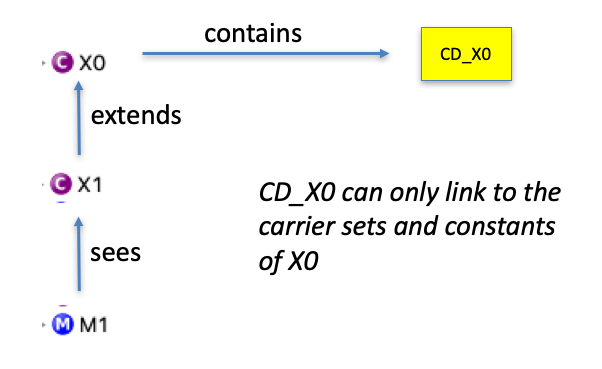
\includegraphics[width=500]{figures/containment_1.png}
		\else
		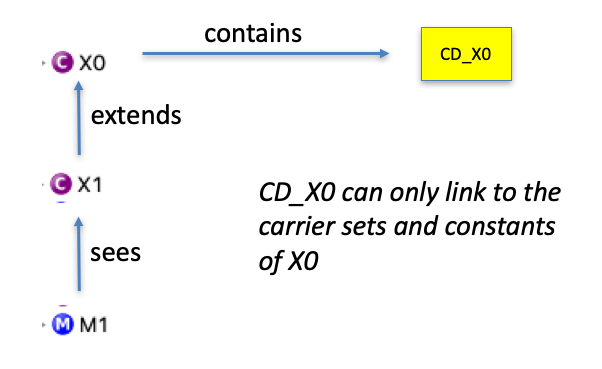
\includegraphics[width=.5\textwidth]{figures/containment_1.png}
		\fi
		\caption{Class Diagram contained in a base level Context}
		\label{fig:CDContainment1}
	\end{figure}
	
	
	\begin{figure}[!htbp]
		\centering
		\ifplastex
		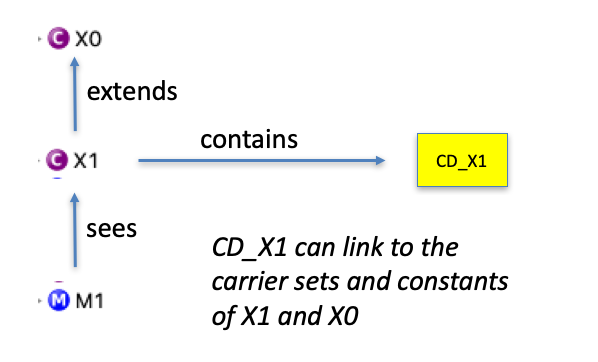
\includegraphics[width=500]{figures/containment_2.png}
		\else
		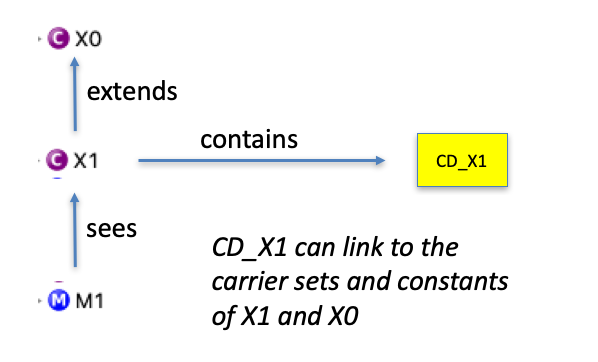
\includegraphics[width=.5\textwidth]{figures/containment_2.png}
		\fi
		\caption{Class Diagram contained in an extended Context}
		\label{fig:CDContainment2}
	\end{figure}
	
	
	\begin{figure}[!htbp]
		\centering
		\ifplastex
		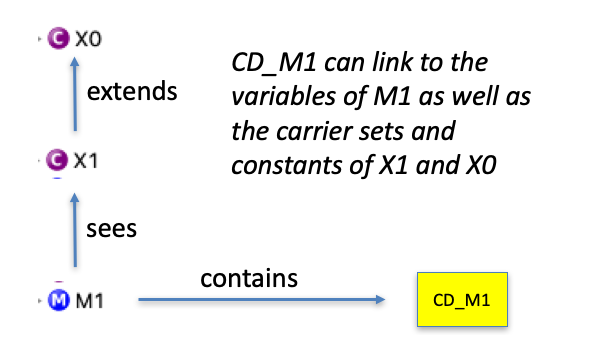
\includegraphics[width=500]{figures/containment_3.png}
		\else
		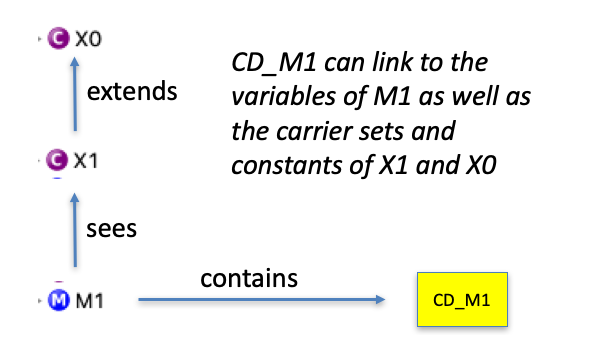
\includegraphics[width=.5\textwidth]{figures/containment_3.png}
		\fi
		\caption{Class Diagram contained in a Machine}
		\label{fig:CDContainment3}
	\end{figure}

The class diagram editor provides a canvas on which to place and populate classes and create relationships between them.
New diagram elements can either be created and populated by selecting the appropriate tool in the palette, or by using the popup tool that appears whenever the cursor is first paused on the canvas or over a diagram node. For example, Fig.~\ref{fig:CDpopups} shows the popup that appears when the cursor is hovered over a \code{class}. 
Similarly, connectors between classes can be drawn using the palette tools or by using the connector handles that appear when the cursor is hovered over a \code{class} (also shown in Fig.~\ref{fig:CDpopups}).

	\begin{figure}[!htbp]
		\centering
		\ifplastex
		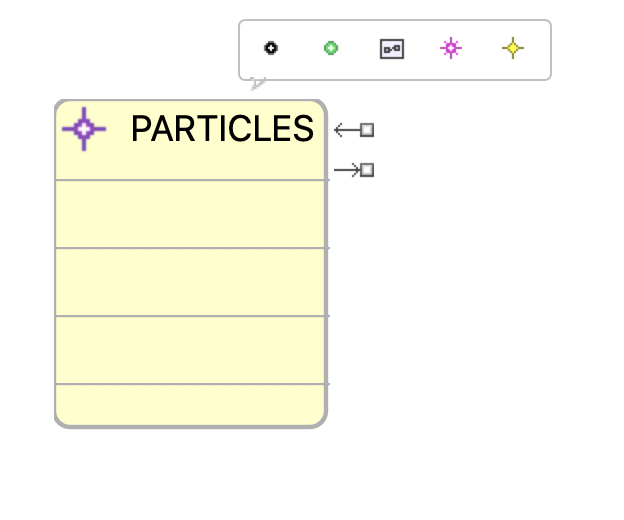
\includegraphics[width=300]{figures/popups.png}
		\else
		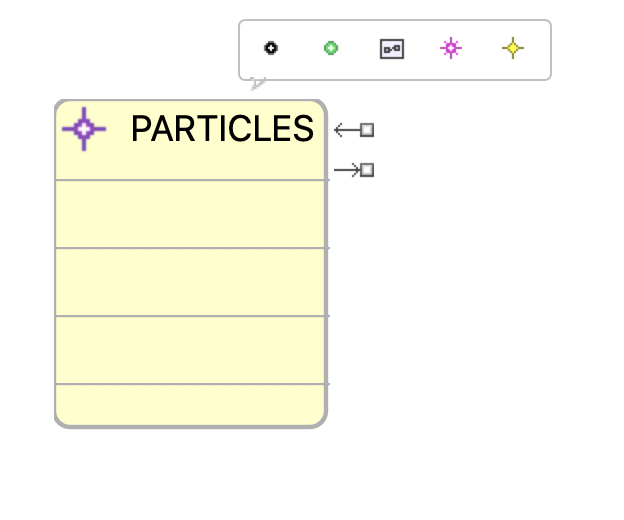
\includegraphics[width=.3\textwidth]{figures/popups.png}
		\fi
		\caption{Class Diagram popups and connectors}
		\label{fig:CDpopups}
	\end{figure}

The class diagram editor provides a context dependent property view which shows and allows editing of the currently selected diagram element.
In fact, much of the modelling takes place on the property sheets rather than the diagram canvas.
All property views default to a top level tab called \code{Overview} which contains the main properties of the diagram element.
This is followed by several tabs that can be used to view the relationships and children of that element.
Where appropriate these tabs allow the relationships and children to be re-ordered in the model.
This is reflected in the translation and can be useful when the order is significant in the generated Event-B.
Finally, following this variable set of tabs, all elements have the following tabs:
\begin{itemize}
	\item \code{model} - a low level access to all fields of the model including those that are not usually exposed to the user.
	\item \code{Rulers \& Grid} - controls that affect the diagram user interface.
	\item \code{Appearance} - controls that affect the rendering of the selected element in the diagram (e.g. colour, font, line style).
\end{itemize}
The more specific properties views for a particular element type will be described in the appropriate sub-sections that follow. 

The property sheet for the class diagram canvas contains the diagram name and a comment field in the \code{Overview} tab and has tabs that list the main details of its classes and associations in a re-orderable table.

\emph{Tip: The tab for classes is particularly important since the translation order can affect guard and invariant ordering which is significant for typing and proving.}


%% subsections for each element type in a class diagram
	
	\section{Classes}
\label{sec:classdiagrams-classes}


	%
	\section{Supertypes of Classes}
\label{sec:classdiagrams-supertypes}

\code{Supertype} relations between classes are drawn using a closed arrow connector on the canvas.
This arrow indicates that the instances of the class at the source of the arrow are a subset of the instances of the class at the target end of the arrow.
Fig.~\ref{fig:ClassSupertypeSimple} shows a class \code{Quarks} that is a subset of (i.e. has a \code{supertype} relationship with) another class, \code{PARTICLES}.
The \code{Supertypes} tab of the class properties lists all of the supertypes  of that class (in this case just the one).


\begin{figure}[!htbp]
	\centering
	\ifplastex
	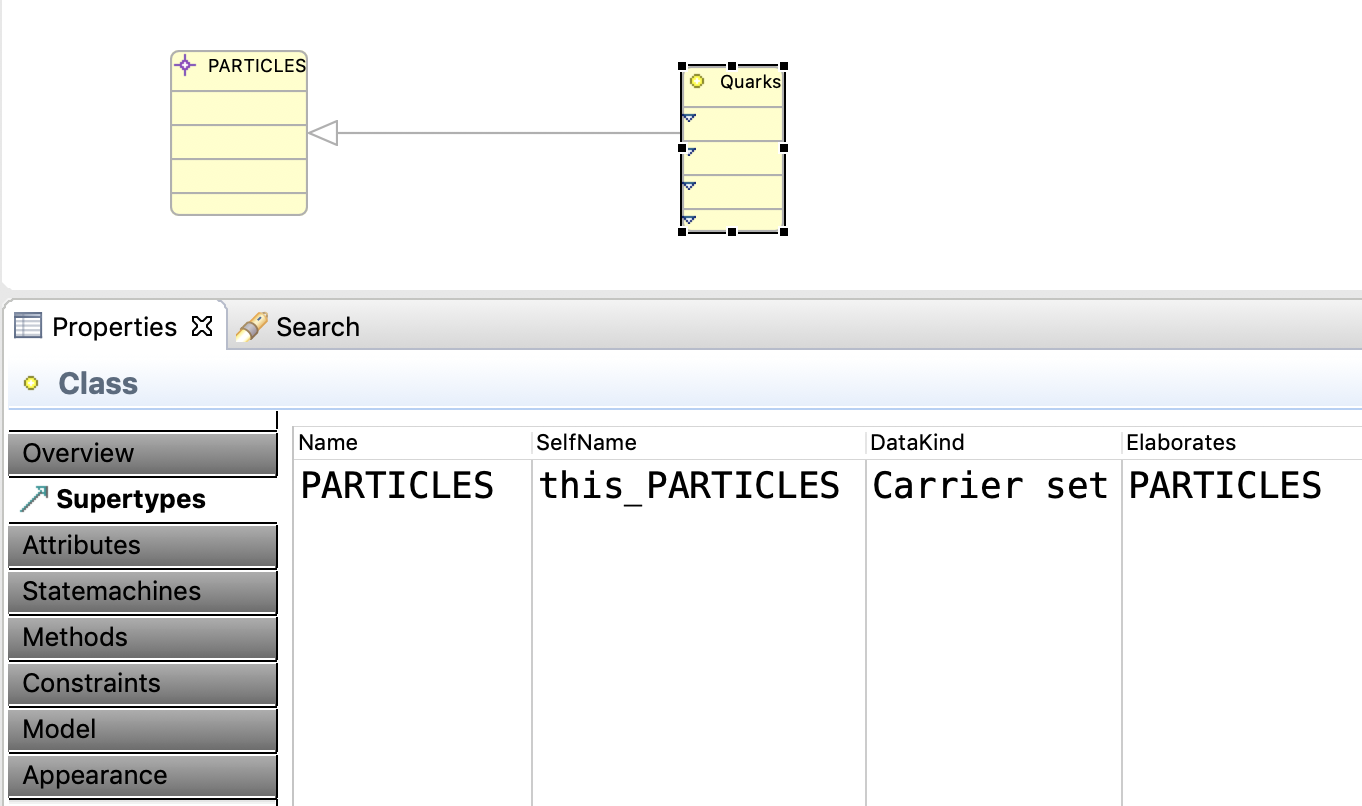
\includegraphics[width=700]{figures/ClassSupertypeSimple.png}
	\else
	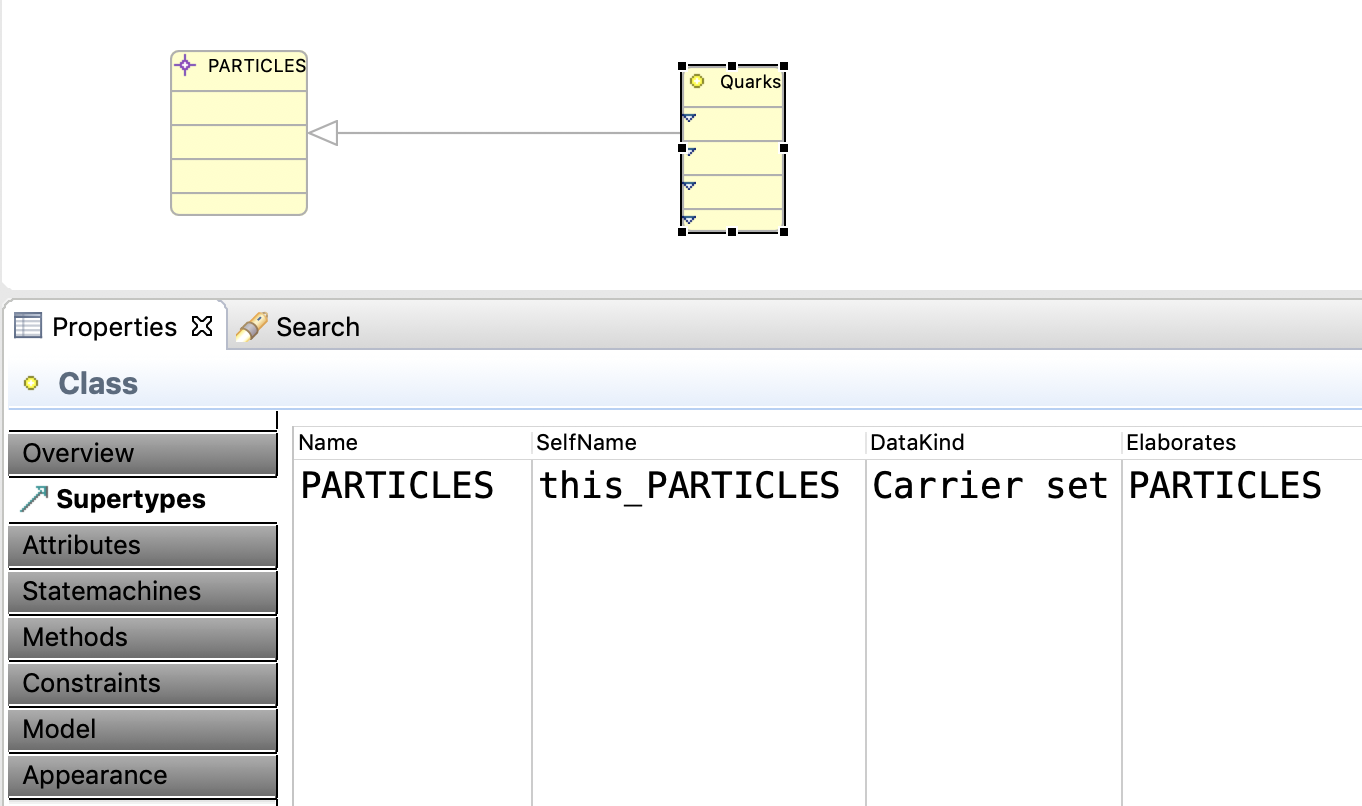
\includegraphics[width=0.7\textwidth]{figures/ClassSupertypeSimple.png}
	\fi
	\caption{Supertype relationship between two classes}
	\label{fig:ClassSupertypeSimple}
\end{figure}

 
\emph{Note: It is more natural to draw supertype relationships on the class diagram, but in Event-B we tend to reverse this relationship and think about subtype relations.
	This is reflected in the translation and also to some extent in the descriptions that follow.}

When several classes have the same supertype the default assumption is that there are no additional constraints to the individual subset relationships. That is, there may be elements of the supertype that are in both subtypes and others that are not in any subtype.
A subtype grouping element is available to specify that a group of subtypes are disjoint, cover all instances or both (partition).
\emph{Note: There is no pallette tool for creating subtype groups; they have to be created using the popup menu for a class. (Use the leftmost icon in the popup shown in Fig.~\ref{fig:CDpopups}).}
Fig.~\ref{fig:ClassSubtypeGroup} shows a group of subtypes and the properties of the group. The default setting is \code{Disjoint} and \code{Cover} (i.e. a partition). The generated Event-B is shown below. 

\begin{figure}[!htbp]
	\centering
	\ifplastex
	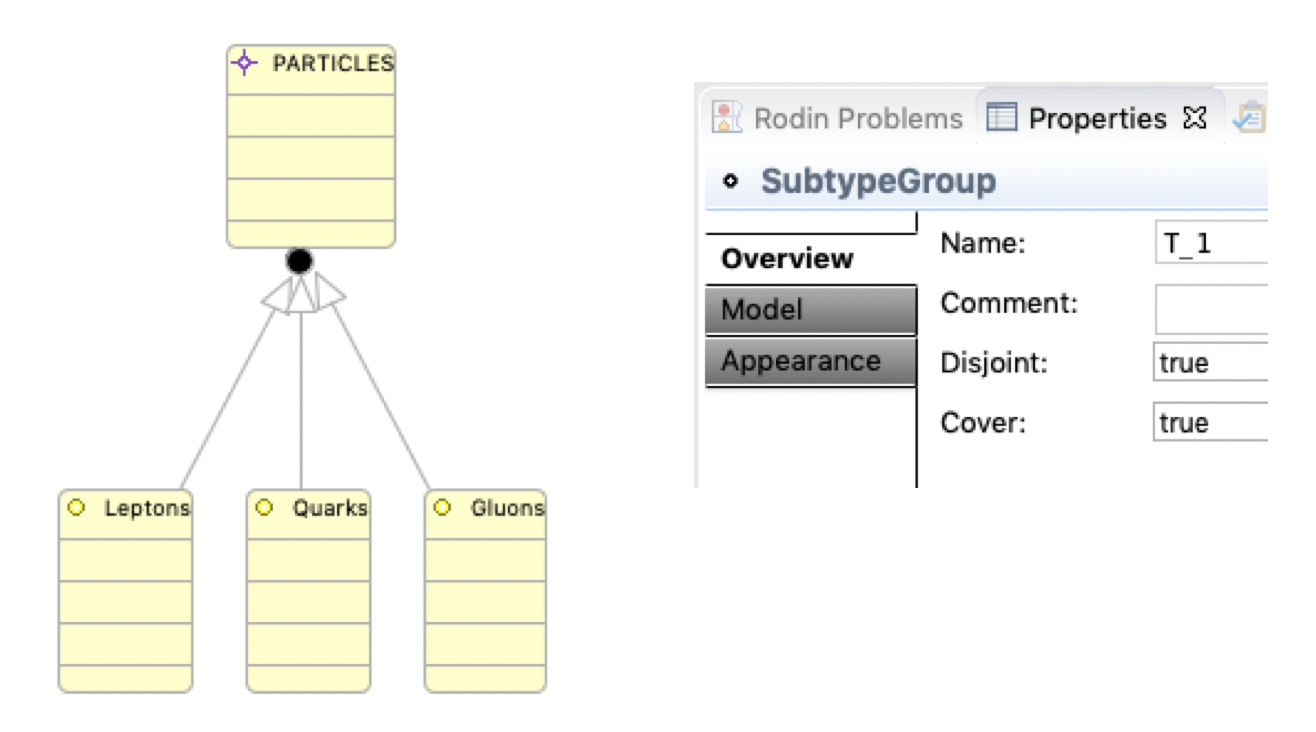
\includegraphics[width=700]{figures/ClassSubtypeGroupPartition.png}
	\else
	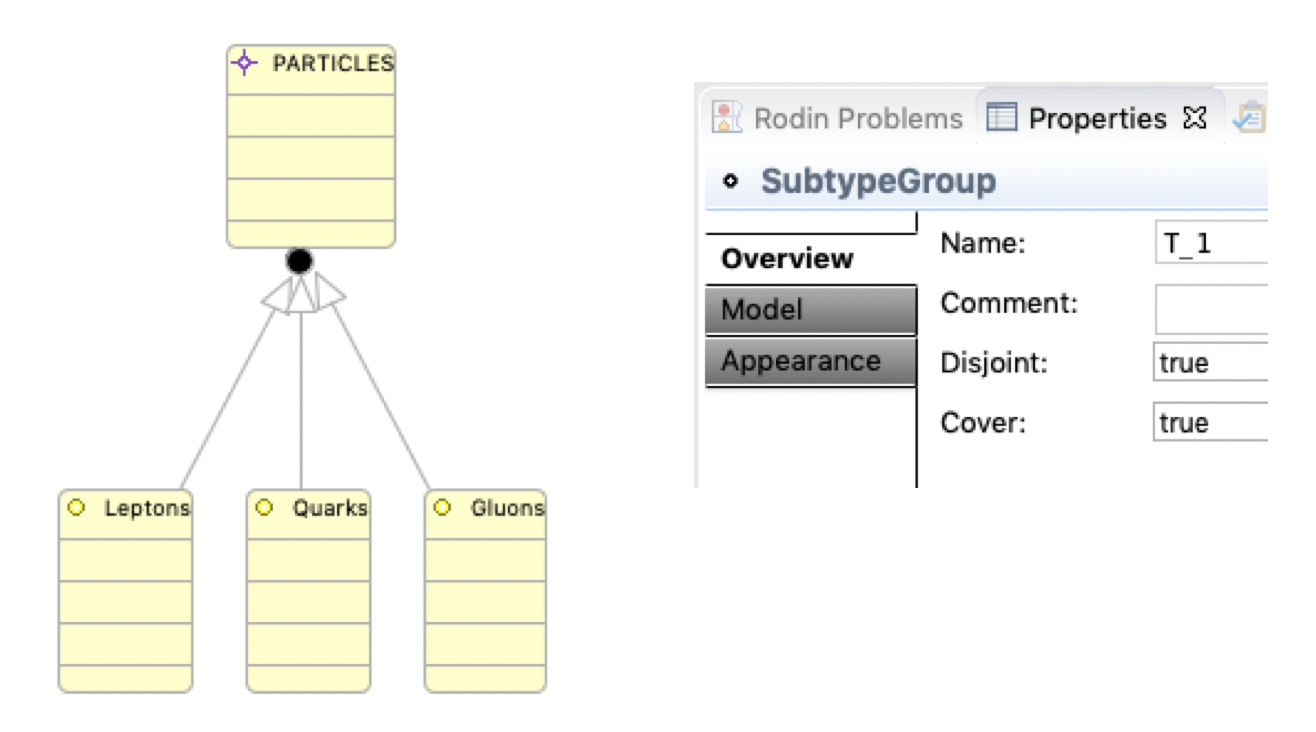
\includegraphics[width=0.7\textwidth]{figures/ClassSubtypeGroupPartition.png}
	\fi
	\caption{Subtype group and its properties}
	\label{fig:ClassSubtypeGroup}
\end{figure}

\CONTEXT{SubtypeGroups}{}{}
\SETS{
	\Set{PARTICLES}{}
}
\CONSTANTS{
	\Constant{Leptons}{}
	\Constant{Quarks}{}
	\Constant{Gluons}{}
}
\AXIOMS{
	\Axiom{subtypeGroup\_T\_1}{false}{$partition(PARTICLES, Leptons, Quarks, Gluons)$}{}
	\Axiom{PARTICLES\_supertypeOf\_Leptons}{false}{$Leptons \in{} \pow{}(PARTICLES)$}{}
	\Axiom{PARTICLES\_supertypeOf\_Quarks}{false}{$Quarks \in{} \pow{}(PARTICLES)$}{}
	\Axiom{PARTICLES\_supertypeOf\_Gluons}{false}{$Gluons \in{} \pow{}(PARTICLES)$}{}
}
\END

When \code{Disjoint = true} and \code{Cover = false}, specifying that the subtypes are disjoint but not a partition, the partition axiom is adjusted to allow for some elements that are in the remainder.
It is also possible to specify \code{Disjoint = false} and \code{Cover = true} giving a predicate over the union of the subtypes.
However, this case is not usually useful.
%\CONTEXT{SubtypeGroups}{}{}
%\AXIOMS{
%		\Axiom{subtypeGroup\_T\_1}{false}{$partition(PARTICLES, Leptons, Quarks, Gluons, PARTICLES\setminus{}(Leptons\bunion{}Quarks\bunion{}Gluons))$}{}
%}
%\END

\emph{Tip: A common use of subtypes is to define a variable class representing the currently created instances, which is a subset of a constant class representing the universe of instances that could possibly exist at some point in time. 
This would be done in a machine resulting in an} \code{invariant} \emph{such as}  $\code{quarks} \in{}  \pow{} \code{(Quarks)}$.
	%
	\section{Associations}
\label{sec:classdiagrams-associations}


	%	
	\section{Class Attributes}
\label{sec:classdiagrams-attributes}



\paragraph{Initial Value } 
The initial value field is a Rodin Keyboard text field. 
The string in the text field is used as the intialisation value for the owning class attribute (or association) but can be interreted in several ways:
\begin{itemize}
	\item If the attribute is owned by a variable instance class, this field is currently ignored. (It should be used in a constructor).
	\item If the attribute elaborates a constant, this field is ignored. 
	\item If the attribute elaborates a variable, an action is added to the Initialisation event to intialise the attribute. as follows:
	\begin{itemize}
		\item if the text field begins with one of the Event-B assignment operators it is used to assign to the complete attribute relation (i.e. expression = attribute.name+initialValue.String)
		\item otherwise the text is assumed to contain the value to be assigned to each and every instance \\(i.e. expression = attribute.name+":="+class.name+"X"+initialValue.String)
	\end{itemize}	
\end{itemize}


%%% Local Variables:
%%% mode: latex
%%% TeX-master: "iuml-b-classdiagrams-user_manual"
%%% End:

	%
	\section{Class Methods}
\label{sec:classdiagrams-methods}
	%
	\section{Class Constraints}
\label{sec:classdiagrams-constraints}

\begin{itemize}
	\item appropriate placement and deciding axiom or invariant

	\item quantification over instances

	\item considerations for ordering and how to fix it

\end{itemize}

	%
	\section{Class Statemachines}
\label{sec:classdiagrams-statemachines}
	%
	\section{Refinement of Class Diagrams}
\label{sec:classdiagrams-refinement}


\begin{itemize}
	
	\item generating a refinement 
	
	\item what it gives you
	
	\item simplification	
	
\end{itemize}
	
\end{document}

%%% Local Variables:
%%% mode: latex
%%% TeX-master: t
%%% End: